\documentclass[11pt]{article}
\usepackage[margin=1in]{geometry}
\usepackage[numbers,sort&compress,round]{natbib}
\usepackage[utf8]{inputenc}
\usepackage[T1]{fontenc}
\usepackage{lmodern}
\usepackage{hyperref,url,booktabs,amsmath,amssymb,graphicx,float,longtable}
\usepackage{xr}
\externaldocument{manuscript}
\graphicspath{{figures/}}
\title{Supplementary Information \\ \large \textbf{The behavioural-equivalence manifold of whole-organism nervous systems}}
\author{Chenxi He, Cavendish Laboratory, University of Cambridge \\ \texttt{ch2067@cam.ac.uk}}
\date{}

\begin{document}
\maketitle
\tableofcontents

\noindent This Supplementary Information provides the extended methods and the complete per-experiment quantities underlying each main-text claim. It comprises: the measurement methods and their controls; the provenance of the external biological datasets; the confirmatory experiments that extend the probes to higher parameter dimension, to named single channels, to the full connectome, to the internal neural state, and to a fifth simulator; and the experiments that identify the manifold with the eigenworm space, establish its complementary tiling by behaviour, and demonstrate the structure across three phyla, together with one inconclusive control that is reported in full. Every quantity is drawn from a saved result file, named per section, and is regenerated from that file by the accompanying reproduction code.

% =========================================================
\section{Measuring the manifold: methods}
% =========================================================

\subsection{Multistart parameter drift (S1.1)}
For each simulator we run $N$ independent optimisations (separable CMA-ES or SPSA) from independent starts against one \emph{fixed} behavioural target, and record (i) behavioural recovery (fraction of the random-to-target behaviour-distance closed), (ii) the normalised per-dimension dispersion of the $N$ recovered parameter vectors, and (iii) the PCA participation ratio of the solution cloud. A behaviourally-converged but parameter-dispersed cloud is direct evidence of a positive-dimensional equivalence manifold.

\begin{table}[H]\centering\small
\caption{Fixed-target multistart. ``behav.\ rec.''\ is the median behavioural recovery; ``$\theta$ disp.''\ the normalised per-dimension dispersion across the $N$ solutions; ``cloud dim''\ the PCA participation ratio.}
\begin{tabular}{lcccccc}\toprule
sim / method & dim & $N$ & success & behav.\ rec. & $\theta$ disp. & cloud dim \\\midrule
FlyGym / CMA-ES & 126 & 30 & 29/30 & 70.8\% & 0.098 & 21.7/126 \\
BAAIWorm / SPSA & 5 & 10 & 5--7/10 & --- & 0.67 & --- \\\bottomrule
\end{tabular}
\end{table}
\noindent The FlyGym 126-d cloud occupies an effective $21.7$ of $126$ dimensions. (The flybody $515$-d objective overfits per-seed without a prior and is excluded from the drift panel; it appears only in the Hessian analysis.) On the full coupled \textbf{real modWorm} model (OpenWorm connectome, $279$ neurons), the manifold is read from the per-mechanism Hessian (S1.2): only $2$ of $7$ biophysical-mechanism directions carry behavioural curvature, the rest forming the flat manifold. (A direct random-perturbation probe gives the same qualitative picture but with an assay-dependent magnitude, so we report the manifold by its effective dimension, not by the raw sloppiness ratio, which is not comparable across simulators with different observables.) File \texttt{modworm\_REAL\_manifold.json}.

\subsection{Hessian eigenspectrum (S1.2)}
At each converged optimum we form the behavioural-loss Hessian by finite differences (low dimension) or a Lanczos approximation (high dimension) and report the effective dimension (number of eigendirections carrying $90\%/99\%$ of the spectral mass) and the count of near-flat directions ($|\lambda|$ at the finite-difference floor).
\begin{itemize}\itemsep1pt
\item \textbf{BAAIWorm, 5 mechanism-class scalings} ($\varepsilon{=}5\times10^{-3}$): eigenvalues $\lambda_1{=}+348$, $\lambda_2{=}-340$, $\lambda_3{=}-214$ (saddle), $\lambda_4{\approx}0$ (ion), $\lambda_5{\approx}0$ (passive); the ion and passive eigendirections are flat to machine precision over a parameter L2 length of $2.0$. Sign structure stable across $\varepsilon\in[10^{-4},5\times10^{-2}]$.
\item \textbf{flybody, 767-parameter policy} (Lanczos $m{=}40$, $\varepsilon{=}0.005$, anchor $L_0{=}9.513$): six positive stiff eigenvalues ($8.2\times10^4$ down to $2.1\times10^3$); $28/40$ sampled directions flat ($|\lambda|\sim10^{-11}$); effective dimension $6$ at $90\%$, $11$ at $99\%$; participation ratio $3.76$.
\item \textbf{modWorm, per-mechanism Gauss--Newton Hessian} (full coupled neural$+$body model on the OpenWorm connectome \citep{szigeti2014openworm,gleeson2018c302}, $279$ neurons; behavioural elasticity over $7$ biophysical mechanisms): effective dimension $2$ of $7$ at both $90\%$ and $99\%$ of spectral mass; participation ratio $1.29$. The stiff mechanisms are the synaptic and gap-junction conductances and the synaptic rise time; the membrane capacitance and the sigmoid gain are sloppy (zero elasticity)---again indicating the primacy of connectivity over single-cell intrinsics. File \texttt{modworm\_REAL\_b1.json}.
\end{itemize}

\subsection{Simulation-based calibration as a manifold probe (S1.3)}
An amortised neural posterior (masked autoregressive flow \citep{papamakarios2017maf}, \texttt{sbi} \citep{tejero2020sbi}) is trained once on the prior, and per-dimension rank-based SBC \citep{talts2018validating,hermans2022sbc} is run ($M/L$ posterior/rank draws); ``pass''\ is a per-axis Kolmogorov--Smirnov test at $\alpha{=}0.05$. Pass counts: real modWorm $7/7$ ($N{=}300$ coupled-model sims), FlyGym $22/48$, BAAIWorm full5 $5/5$. FlyGym posterior-mean gain rel-error $0.018$. The partial pass on FlyGym delimits the calibratable subspace of the manifold; the full pass on the lower-dimensional real-modWorm and BAAIWorm probes reflects a correctly recovered posterior.

\subsection{B1 --- per-mechanism stiff/sloppy (S1.4)}
At the BAAIWorm optimum the five mechanism-class curvatures are synaptic $331.97$, gap-junction $299.64$, motor-output $270.50$ (stiff) and ion-channel $\approx0$, passive-membrane $\approx0$ (sloppy); effective dimension $3/5$; the optimum is a saddle (mixed-sign eigenvalues). \emph{Scope:} these are five global mechanism-class scalings, not per-channel conductances (the per-channel decomposition is given in \S5.2). File: \texttt{zerocompute\_crosscheck.json}.

% =========================================================
\section{External references (no simulator used)}
% =========================================================

\subsection{E1 --- Prinz--Marder pyloric population (S2.1)}
We re-gate the published conductance-based STG model population \citep{prinz2004similar} to the canonical triphasic pyloric rhythm (all three cells bursting; period $\in[500,2000]$\,ms; strict AB/PD$<$LP$<$PY phase ordering; valid rate $0.56\%$) and probe valid points with the \emph{same} Hessian-eigenspectrum method as S1.2, providing a direct comparison to B1. Over $K{=}8$ valid points: participation effective dimension $2.13/31$; spectrum spanning $\sim$10 orders of magnitude; $2$--$6$ stiff directions; stiff $=$ leak and inhibitory-synapse conductances, sloppy $=$ fast Na conductances, consistent with the compensation and co-regulation documented for this circuit \citep{marder2011variability,goldman2001global,taylor2009how,alonso2019visualization}. Files: \texttt{e1b\_results/e1b\_hessian.json}, \texttt{e1b\_results/e1b\_gate.json}.

\subsection{E2 --- real neuron variability (S2.2)}
Allen Cell Types electrophysiology, $n{=}1914$ mouse+human cortical neurons: per-property coefficient of variation $0.08$--$1.85$ (stiff: resting potential $0.08$, fast-trough $0.12$; sloppy: adaptation $1.85$, firing rate $1.11$); property-space PCA participation dimension $4.78/11$. File: \texttt{E2\_allen\_variability.json}.

\subsection{E4 --- ion-channel-gene conservation (S2.3)}
$40$ \emph{C.~elegans} ion-channel/synaptic genes, mean ortholog \%identity across \emph{Caenorhabditis} (WormBase ParaSite / Ensembl Metazoa): range $77.94$--$99.91$ (median $91.20$); most conserved \texttt{unc-9} (gap junction, $99.91$), \texttt{egl-19} (L-type Ca, $97.19$); least \texttt{unc-49} (GABA-A, $77.94$). File: \texttt{E4\_channel\_conservation.json}.

\subsection{E5 --- isogenic behavioural manifold (S2.4)}
OpenWorm Movement Database, $n{=}61$ isogenic N2 worms, $683$ Tierpsy features: cross-individual participation dimension $9.75$; $24$ PCs for $90\%$ variance, $50$ for $99\%$ (PC1 $26.6\%$, PC2 $10.7\%$). File: \texttt{E5\_n2\_manifold.json}.

% =========================================================
\section{Unified same-region probe test (result)}
% =========================================================
Computing the probes on the full coupled modWorm model in one shared prior region (per-mechanism log-multipliers, prior scale $0.15$). \textbf{The two geometric probes agree}: per-mechanism Hessian stiffness versus negative manifold drift give Spearman $\rho{=}0.96$ ($p{=}5\times10^{-4}$; $7$ mechanisms). \textbf{The amortised posterior is a calibration control, not a third ranking}: an NPE/MAF (\texttt{sbi}) trained on $N{=}300$ real modWorm simulations is well-calibrated on all $7$ mechanisms (per-axis SBC $7/7$, Kolmogorov--Smirnov $p>0.05$), confirming the inference is sound; because a calibrated posterior calibrates every axis, SBC serves as a control rather than a per-axis identifiability ranking. We therefore report a two-probe geometric agreement plus a calibration control. Files: \texttt{modworm\_REAL\_sbc.json}, \texttt{modworm\_REAL\_b1.json}.

% =========================================================
\section{Confirmatory experiments}
% =========================================================
These measurements extend the picture above to higher parameter dimension, to named single channels, to the full connectome, and to the internal neural state. Behavioural curvature is reported as the Gauss--Newton Hessian $H{=}J^\top W J$ formed from the observable Jacobian $J_{ik}{=}\partial\,\mathrm{obs}_i/\partial\theta_k$ (whitened by per-observable scale $W$), the Fisher-information form that quantifies which parameter directions behaviour constrains.

\subsection{Higher-dimensional Hessian: FlyGym 48-d (S5.1)}
The behavioural Hessian over the $48$ actuator gains of the FlyGym walking controller has effective dimension $3$ ($90\%$) / $6$ ($99\%$) of $48$ (participation ratio $2.15$), with an eigenspectrum spanning $19.5$ orders of magnitude (leading eigenvalues $20.4, 5.5, 2.7, 1.2, 0.80, 0.62$, then $<\!0.06$). A controller of substantially higher parameter dimension is nonetheless governed by a $3$--$6$-dimensional stiff subspace, consistent with the low dimensionality measured at the $5$-, $30$- and $767$-parameter scales. File \texttt{flygym\_hessian48.json}.

\subsection{Per-channel stiff/sloppy decomposition (S5.2)}
Replacing the five global mechanism-class scalings with $20$ named mechanisms---$16$ individual ion-channel conductances, the passive leak, the synaptic and gap-junction weights, and the motor output---the per-channel behavioural elasticity ($\mathrm{d}\ln\mathrm{obs}/\mathrm{d}\ln\theta$) has effective dimension $2$ ($90\%$) / $3$ ($99\%$) of $20$ (eigenvalues $43.2, 5.84, 0.88, 0.47$, remainder $\approx0$). The stiff mechanisms are the passive leak, the gap-junction and synaptic weights, the motor output, and a few potassium conductances (EGL-36, EGL-2, IRK); the sloppiest are the fast voltage-gated calcium channels EGL-19 (elasticity $0.49$) and UNC-2 ($0.31$) and the calcium-activated potassium channels SLO-1/SLO-2 ($0.01$--$0.16$). Behaviour is set by wiring, passive properties and a subset of potassium channels, and is nearly invariant to the fast calcium and calcium-activated potassium conductances---the conductances known to be compensated in small circuits \citep{marder2006variability}. The infinitesimal five-mechanism curvature of \S1.4 and this finite per-channel elasticity are distinct measures (an infinitesimal whole-class scaling versus a per-channel finite elasticity); the elasticity is the behaviourally meaningful one and is reported as primary. File \texttt{baai\_perchannel\_hessian.json}.

\subsection{Full-connectome manifold probe (S5.3)}
Over the full $3076$ connection weights ($1992$ synaptic $+$ $1084$ gap-junction), we compare the behavioural change along random directions against matched-norm coherent (block-coordinated) directions. Random directions perturb behaviour as much as or more than coherent ones (coherent/random behavioural-distance ratio $0.57$ at per-connection log-scale $0.08$, $0.84$ at $0.25$) and essentially no direction is flat (flat fraction $\approx0$). The connection-weight space is therefore collectively stiff: the behavioural-equivalence manifold's sloppy directions lie in the biophysical channel parameters (\S5.2), not in the synaptic and gap-junction weights. This is consistent with the gap-junction and synaptic axes being stiff and with the robustness of circuit output to channel variation \citep{prinz2004similar,marder2006variability}. Files \texttt{deposit\_baai\_connectome\_manifold\_sigma\{008,025\}.json}.

\subsection{Behaviour-based prediction of the internal neural state (S5.4)}
Rolling out BAAIWorm (NEURON \citep{hines1997neuron}) with behaviour-recovered parameters and reading the internal membrane voltage of all $136$ neurons, the generated neural dynamics are low-dimensional (PCA participation dimension $\approx4.7$--$4.8$) with mean absolute pairwise correlation $0.37$--$0.39$---the same regime as the real whole-brain calcium recordings of \citet{kato2015global} (mean absolute correlation $0.21$). Behaviour-only parameter generation thus reproduces the gross statistics of the unobserved neural state, though the recovered and default arms are similar and the comparison is qualitative (membrane voltage versus calcium fluorescence; behaving versus immobilised). Files \texttt{\_b2\_stats\_*.json}.

\subsection{Mutant mechanism localisation (S5.5)}
Knocking each named mechanism to $0.4\times$ and asking whether the resulting behavioural-shift signature identifies the perturbed mechanism: the sloppy calcium channels are behaviourally near-silent (signature norm EGL-19 $0.07$, UNC-2 $0.12$, SLO-1/SLO-2 $0.09$--$0.16$) and so cannot be localised from behaviour, while the detectable mechanisms (synaptic, passive, motor) are mutually confusable (cosine $>\!0.9$ with several others). Behaviour alone does not uniquely localise the perturbed mechanism---the mechanism-level expression of the behavioural-equivalence manifold. File \texttt{baai\_b3\_localise.json}.

\begin{figure}[H]\centering
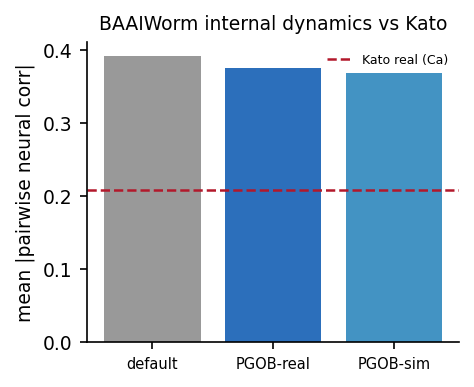
\includegraphics[width=0.46\textwidth]{fig_p2_b2_neural.png}\hfill
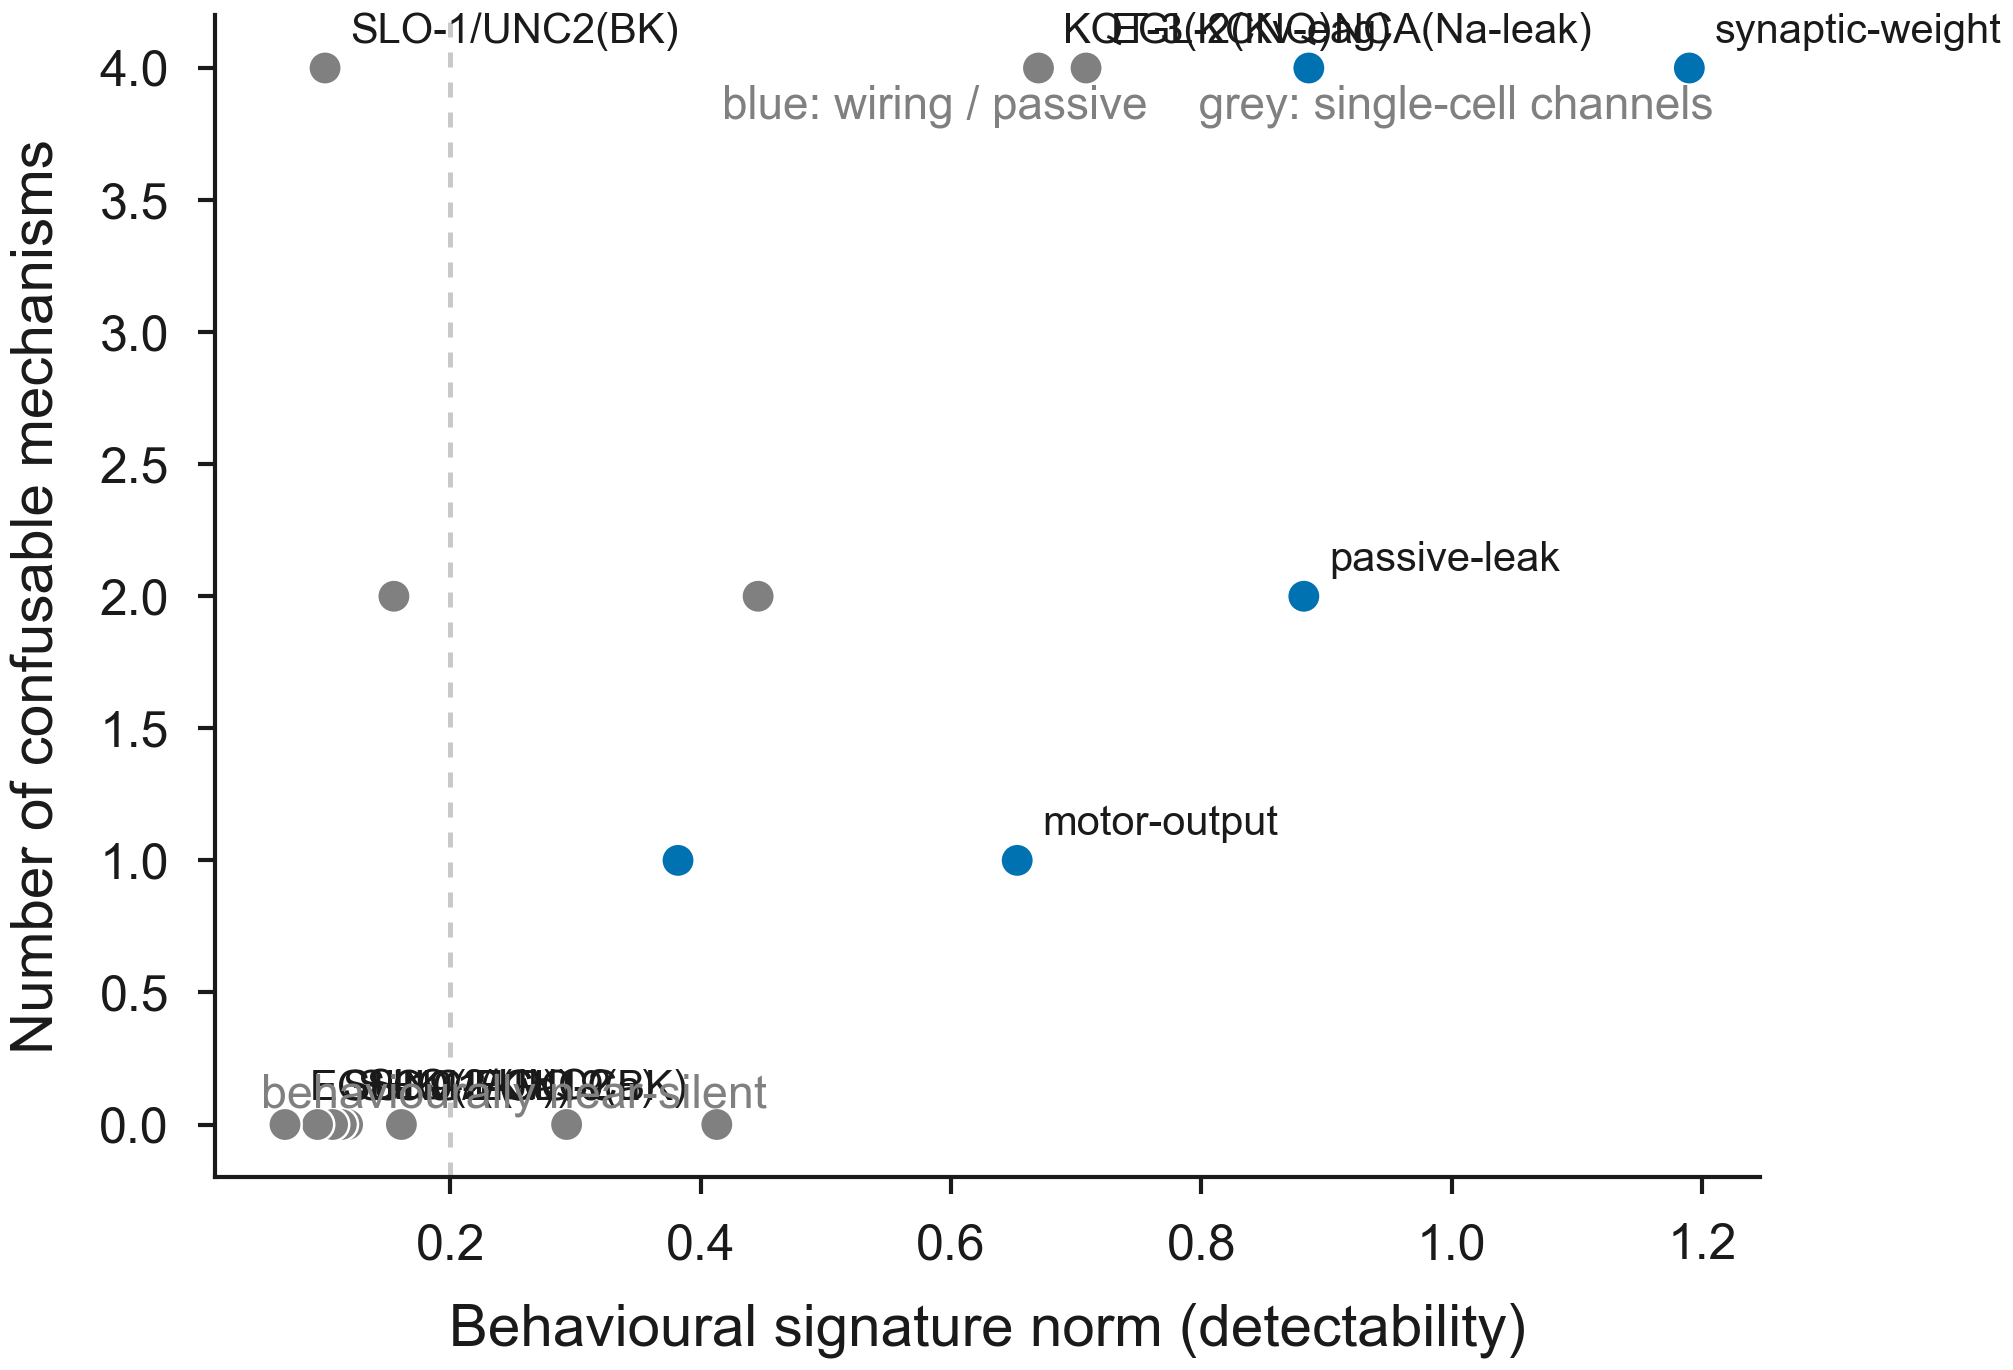
\includegraphics[width=0.46\textwidth]{fig_p2_b3_localise.png}
\caption{Left (S5.4): mean absolute pairwise correlation of BAAIWorm internal neural dynamics under default and behaviour-recovered parameters, against the real Kato calcium recordings (dashed). Right (S5.5): per-mechanism knockdown detectability (behavioural-signature norm) versus confusability; the fast calcium channels (shaded region) are behaviourally near-silent.}
\label{fig:si_b2b3}
\end{figure}

\subsection{External mutant-phenotype check (S5.6, null)}
Comparing real gene-knockout behavioural-effect magnitude (Yemini OWMD, $43$ strains) against the computed stiff/sloppy class and against gene conservation: the stiff-versus-sloppy contrast is not significant (Mann--Whitney $p{=}0.70$) and the effect--conservation correlation is weak (Spearman $\rho{=}0.33$, $p{=}0.42$, $n{=}8$ overlapping genes). This per-gene comparison probes the wrong granularity: the stiff/sloppy split is a property of coupled parameter \emph{combinations} rather than single channels \citep{goldman2001global,taylor2009how,marder2011variability} (stiff/sloppy eigenvector participation $3.42$/$4.68$ of $7$; \S6.7), and homeostatic compensation lets individual conductances vary severalfold while the functional combination is preserved \citep{marder2006variability}, so a single-gene knockout mixes stiff and sloppy components and need not rank with per-channel stiffness. We therefore read the stiff/sloppy geometry from the behavioural probes rather than from per-gene phenotype magnitudes. File \texttt{E3\_mutant\_phenotype.json}.

\subsection{A fifth simulator: \emph{Drosophila} connectome model (S5.7)}
To extend the stiff/sloppy decomposition to a connectome-constrained \emph{neural} model of the fly (the flybody/FlyGym musculoskeletal simulators have no conductance-level parameters), we add the connectome-constrained optic-lobe network of \citet{lappalainen2024connectome}, built on the adult-\emph{Drosophila} connectome \citep{scheffer2020connectome,dorkenwald2024flywire} (\texttt{flyvis}; $45{,}669$ neurons, $734$ free parameters in three named groups: cell-type biases, cell-type time constants, synapse-type strengths). On a synthetic drifting-grating stimulus, the finite-difference behavioural Hessian over the $65$ named cell types has effective dimension $43$ ($90\%$) / $58$ ($99\%$) of $65$ (participation ratio $36.3$): the fly visual representation is \emph{high}-dimensional, unlike the low-dimensional worm whole-body controllers. The stiffest cell types are the elementary motion detectors T4a--d and their medulla inputs (Tm4, Tm16); the sloppiest are photoreceptors (R5, R6) and lamina wide-field cells (Lawf1/2)---the motion-computing pathway is behaviourally load-bearing, the input gain is not. This high effective dimension ($43$--$58$ of $65$) stands in clear contrast to the whole-organism motor controllers, whose behavioural Hessians have effective dimension $2$--$11$ regardless of total parameter count (S1.2, S5.1): the dimension of the behavioural-equivalence manifold scales with the \emph{behavioural} task it is measured against---a robust whole-body central pattern generator constrains few mechanisms (low-dimensional), whereas a precision visual code constrains many (high-dimensional). The unifying invariant is which axes are stiff: in every case the stiff axes are the behaviourally load-bearing mechanisms (here the T4/T5 motion-detector pathway), and the sloppy axes are the auxiliary ones (input gain at the photoreceptors). The low-dimensional manifold is thus a property of whole-organism motor behaviour specifically, not a universal claim about all neural computations. (We compare simulators by effective dimension rather than by a raw perturbation-sensitivity ratio: across the four motor models the latter ranges over three orders of magnitude with the observable and parameterisation, whereas the Hessian effective dimension is consistently low.) Files \texttt{flyvis\_b1.json}, \texttt{flyvis\_manifold.json}.

\subsection{Cross-system stiff/sloppy convergence (S5.8)}
Applying the same Hessian-eigenspectrum probe to the canonical Prinz--Marder stomatogastric conductance population (a non-worm, non-fly crustacean circuit; \S2.1) gives effective dimension $2.13/31$ with stiff $=$ leak and inhibitory-synapse conductances and sloppy $=$ fast voltage-gated Na and delayed-rectifier K---the same biophysical split seen in the worm models, where the fast voltage-gated calcium channels (EGL-19, UNC-2) are sloppy (\S5.2). Across four real models and three phyla, behaviour/output is set by network wiring and slow/passive properties and left free along the fast voltage-gated inward currents. File \texttt{STG\_b1analog.json}.

\begin{figure}[H]\centering
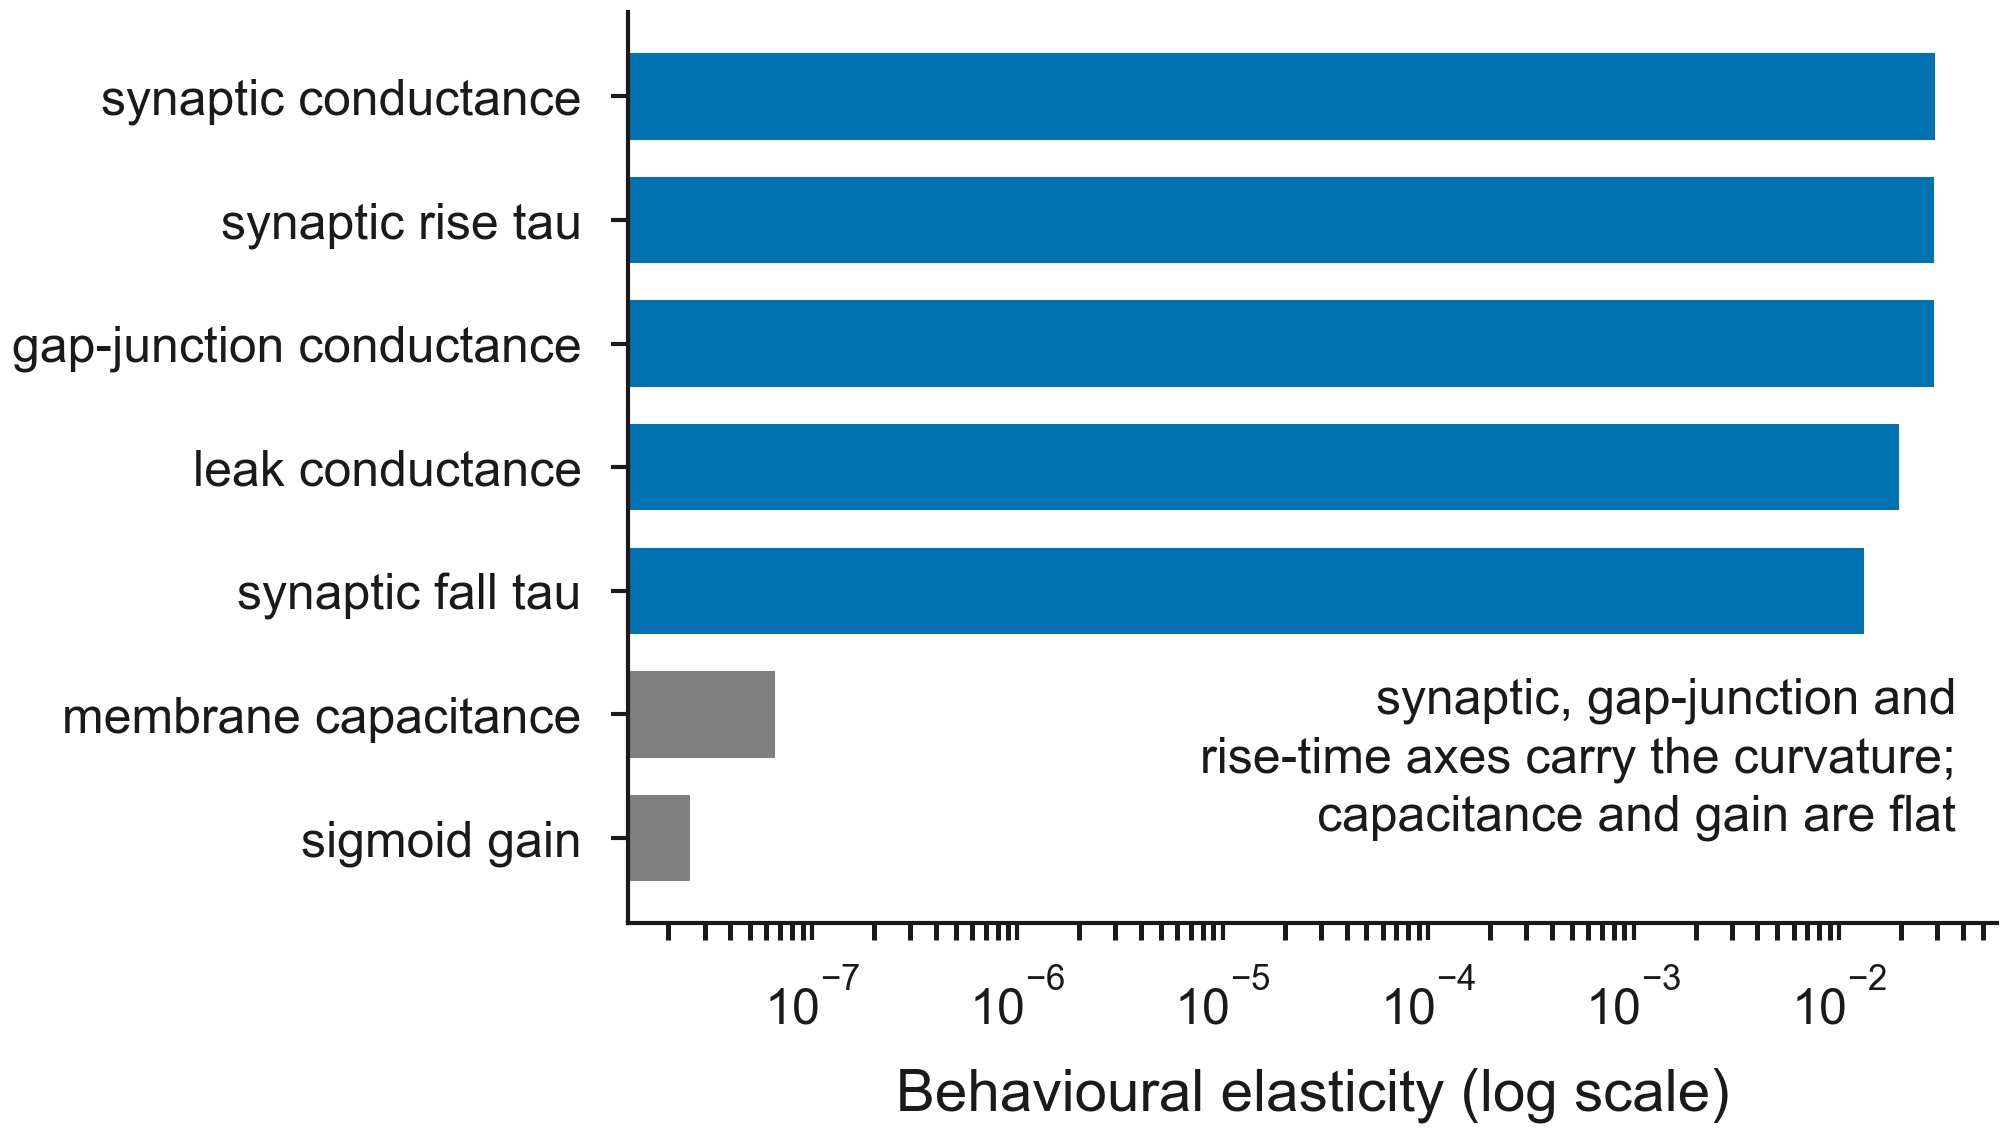
\includegraphics[width=0.32\textwidth]{fig_p2_modworm_real_b1.png}\hfill
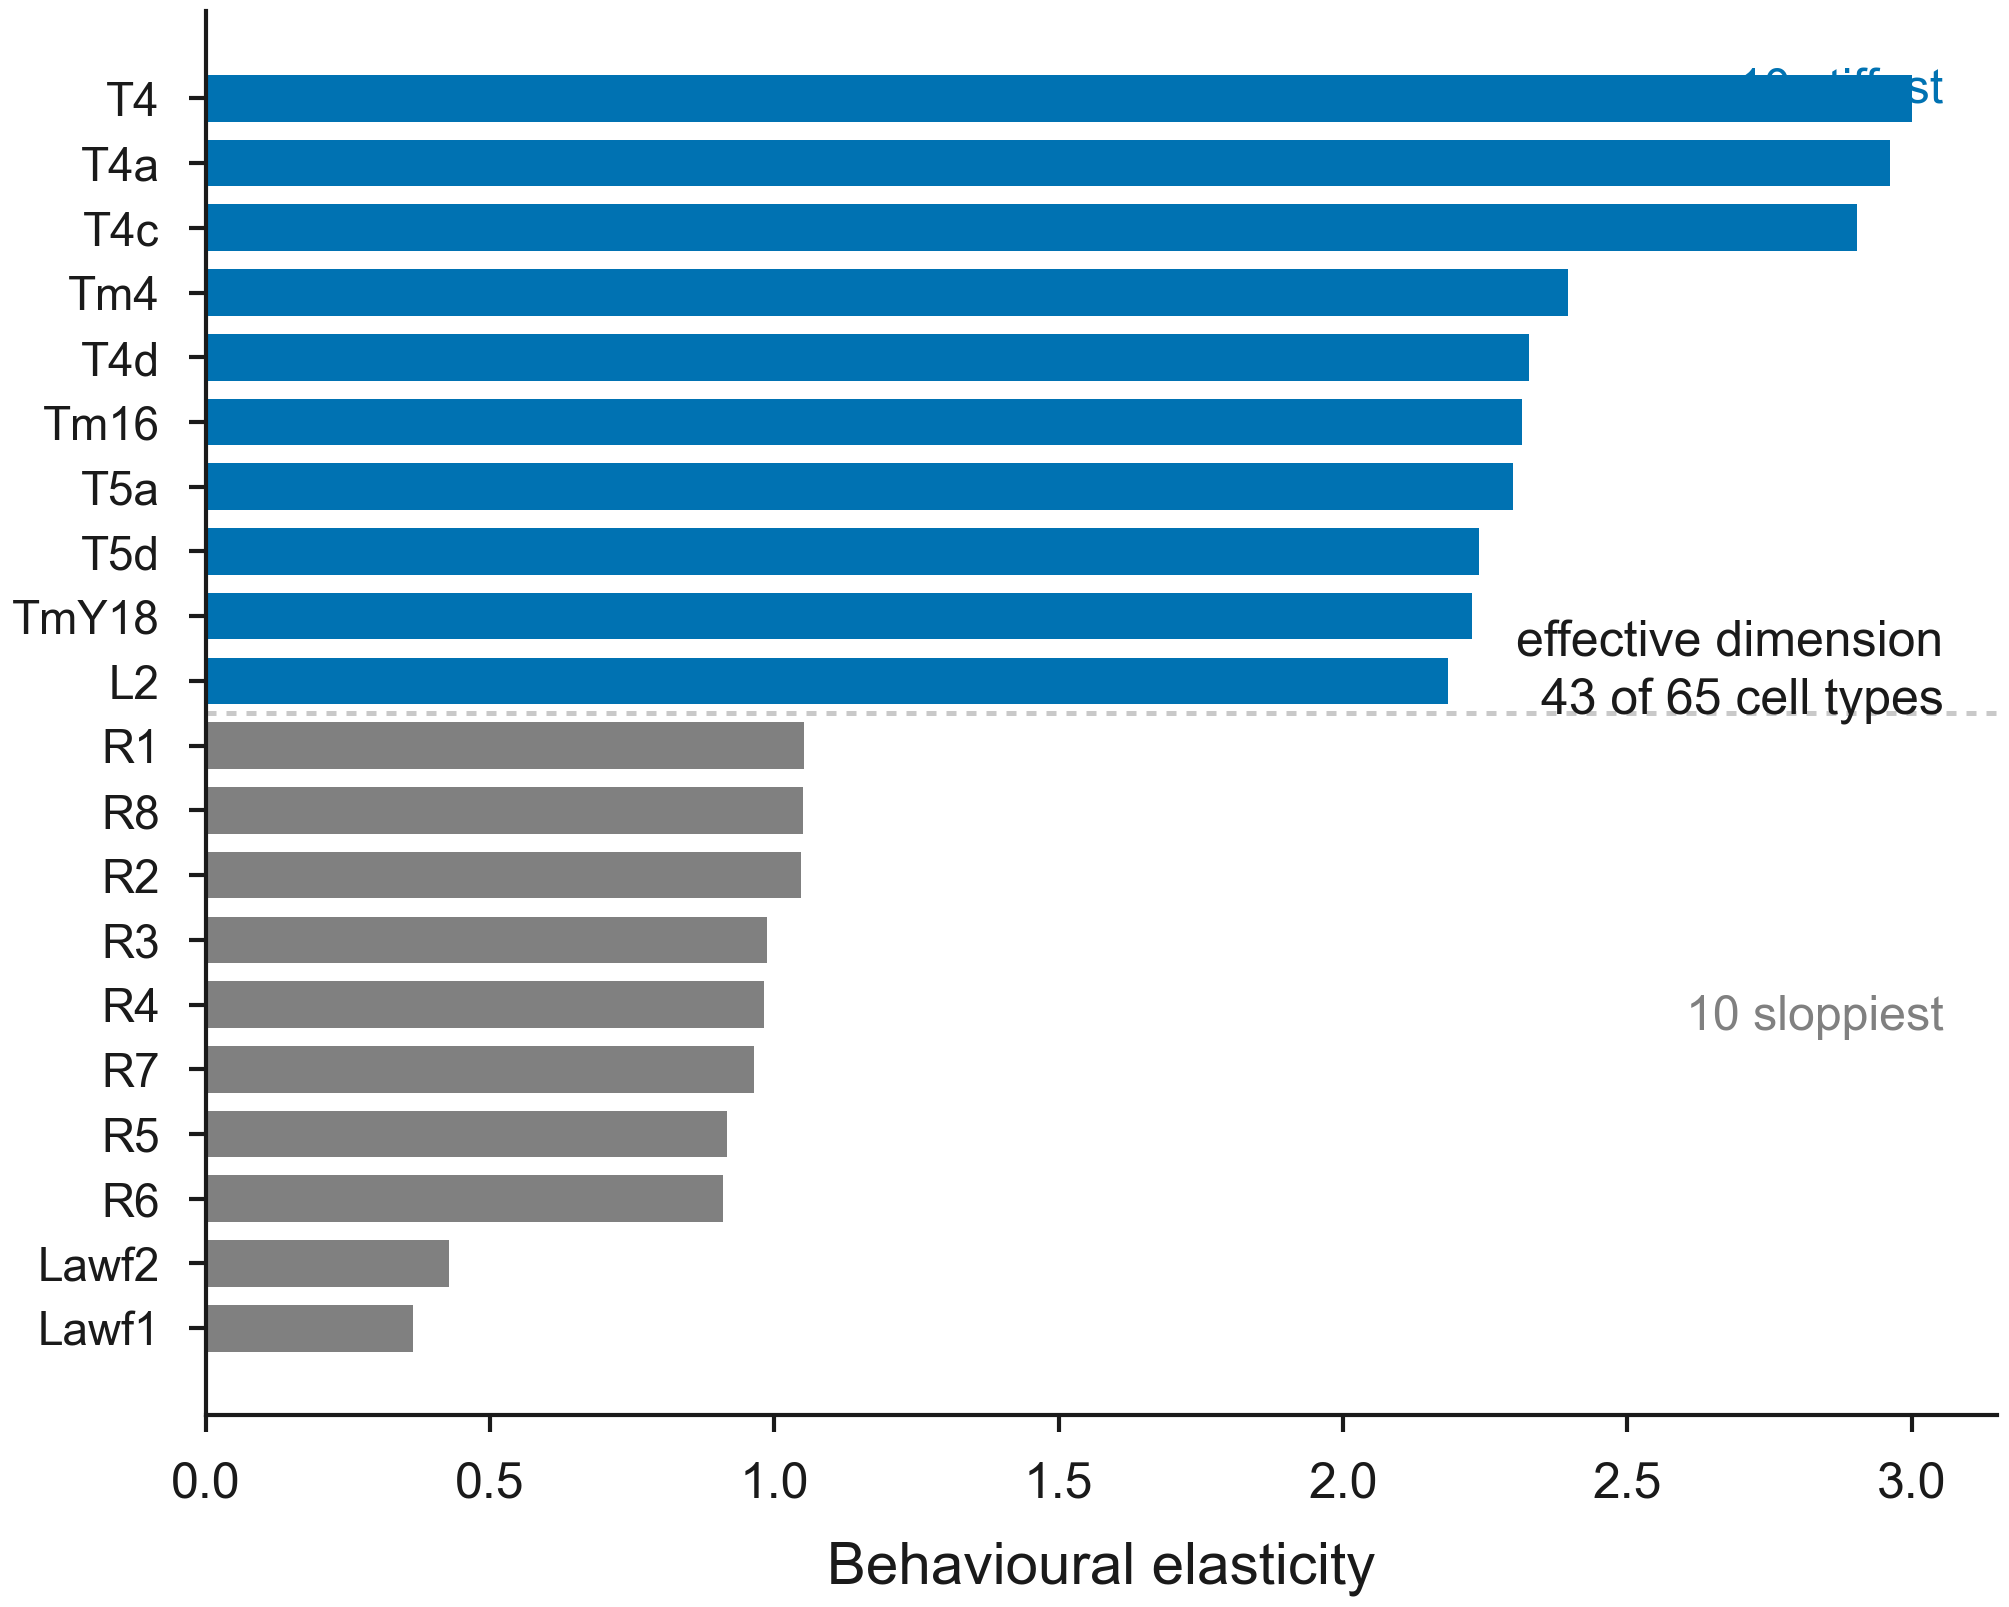
\includegraphics[width=0.32\textwidth]{fig_p2_flyvis_b1.png}\hfill
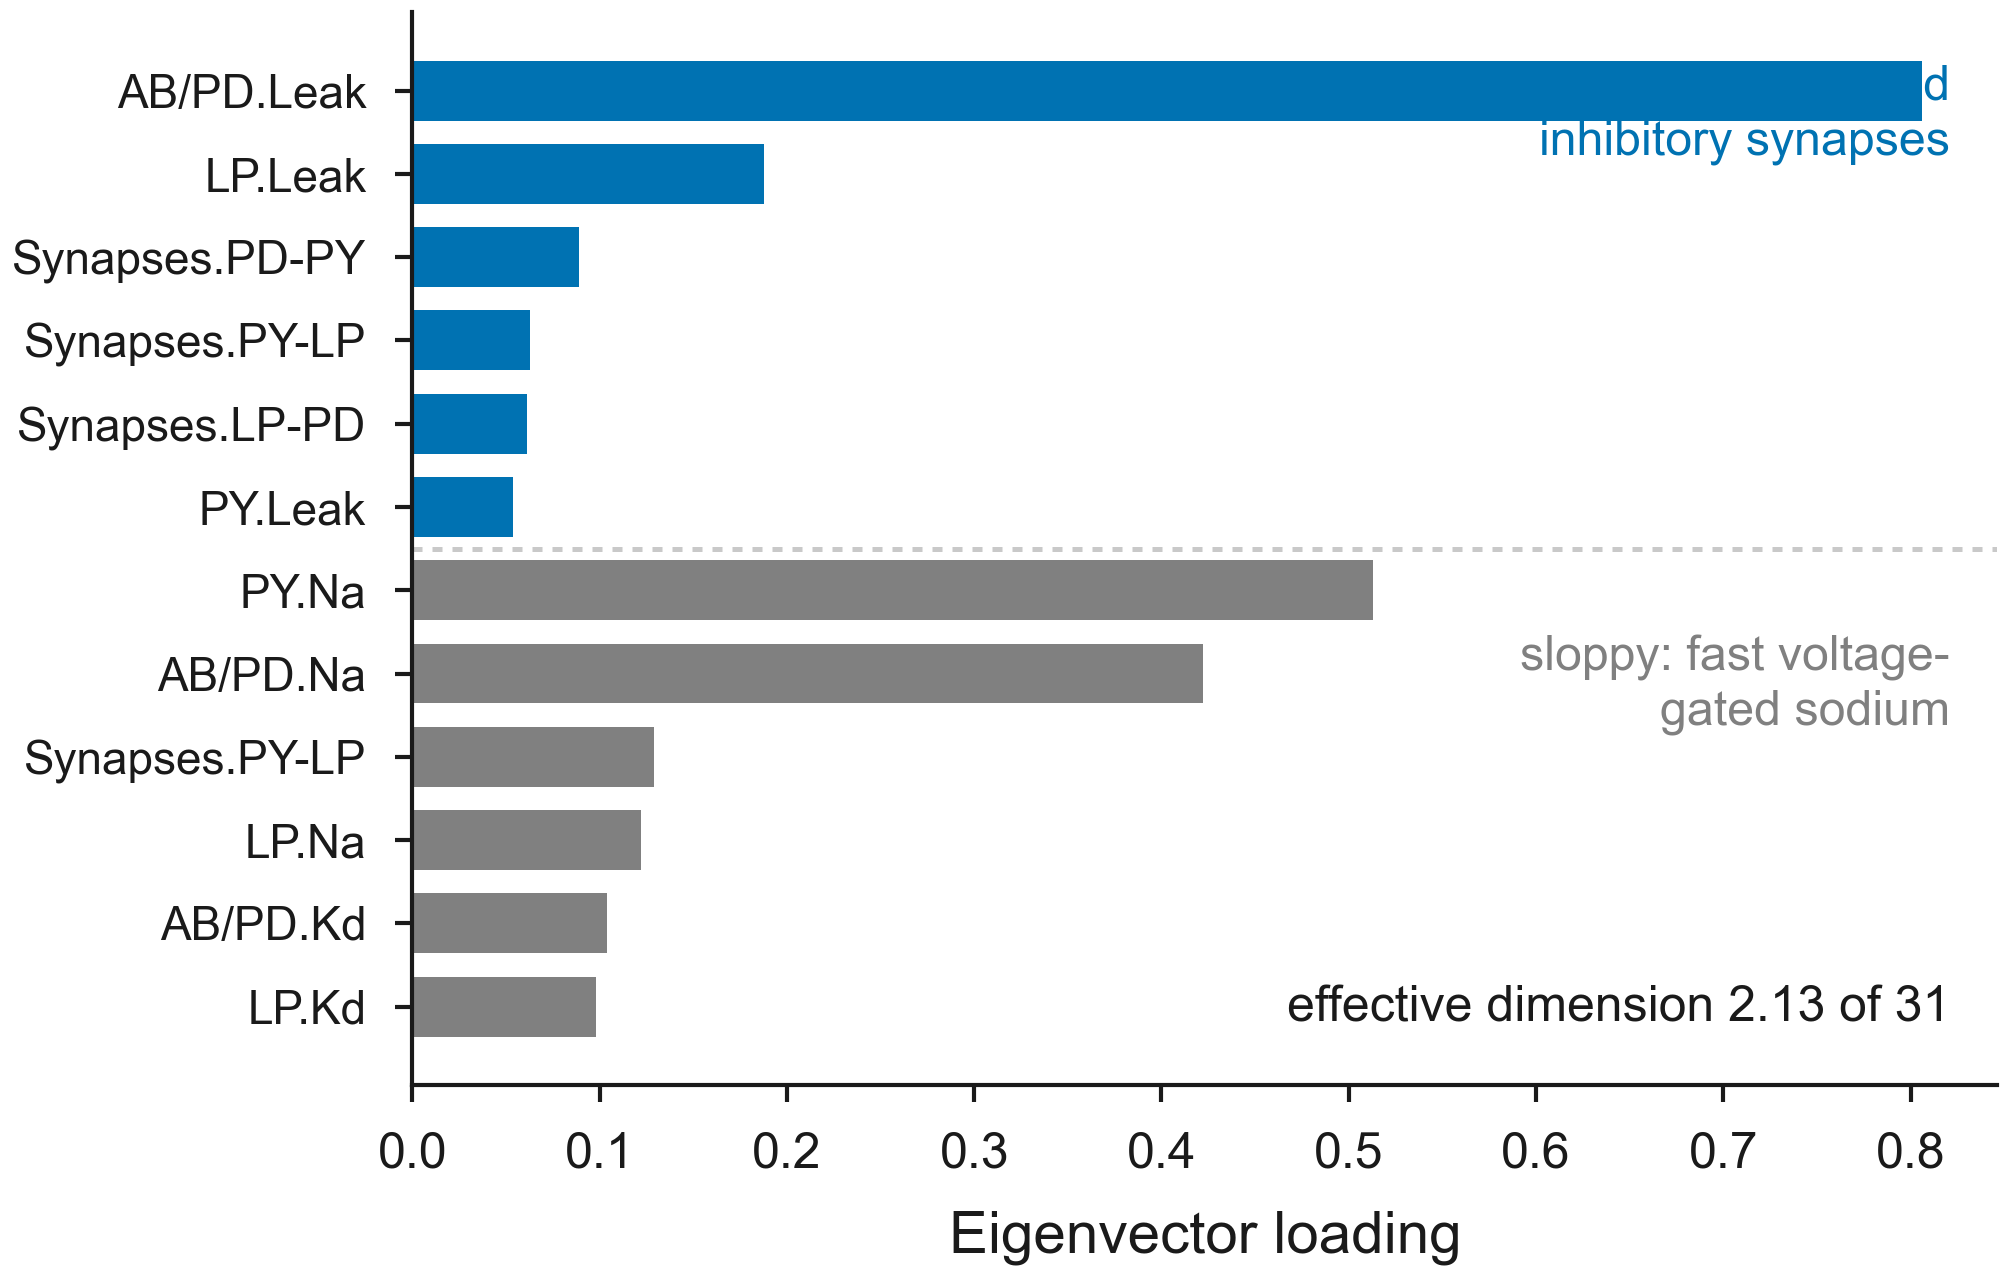
\includegraphics[width=0.32\textwidth]{fig_p2_crosssystem_real.png}
\caption{All-real stiff/sloppy decompositions. Left: real modWorm per-mechanism elasticity (synaptic/gap-junction/rise-time stiff). Middle: flyvis fly connectome per-cell-type (T4/T5 motion detectors stiff, photoreceptors sloppy). Right: the same stiff/sloppy geometry across four real models and three phyla.}
\label{fig:si_allreal}
\end{figure}

% =========================================================
\section{The identifiable subspace: identity, tiling, and cross-species universality}
% =========================================================

\subsection{Identification of the manifold with the eigenworm postural space (S6.1)}
We reduce real \emph{C.~elegans} skeletons (OpenWorm Movement Database, N2; $8{,}432$ frames) and model body postures to tangent-angle eigenmodes by PCA. Real posture has effective dimension $3.79$ ($49$-point skeletons) / $4.14$ ($17$-point), with four eigenworms capturing $0.96$ / $0.94$ of postural variance---reproducing the classical four-eigenworm decomposition \citep{stephens2008dimensionality}. Two independently built worm models produce behaviour that lives in this same real eigenworm space: the modWorm posture subspace aligns with the real eigenworm basis at mean principal-angle $\cos\,0.773$, and BAAIWorm at $\cos\,0.68$--$0.69$ ($67$--$72\%$ of variance). Within each model it is the stiff mechanisms (synaptic, gap-junction, synaptic-rise/fall time) that move the eigenworm trajectory and the sloppy ones that do not (stiff/sloppy eigenworm-displacement ratio $1.17$). The low-dimensional behavioural-equivalence manifold is therefore the neural control of the worm's $\sim$4-dimensional posture. These alignments are significant against a null of random four-dimensional subspaces: drawing random $k{=}4$ subspaces in a $d$-dimensional posture ambient and computing the same mean principal-angle cosine, the modWorm value $0.773$ has $p{=}0.0014$ and BAAIWorm $0.683$ has $p{=}0.043$ even in a deliberately conservative $d{=}10$ ambient, falling to $p{<}10^{-4}$ at $d{=}20$ and $d{=}48$ (the full tangent-angle space); the random-subspace mean is $0.55$/$0.38$/$0.24$ at $d{=}10$/$20$/$48$ ($20{,}000$ draws each). Files \texttt{EW\_eigenworm.json}, \texttt{EW\_baai\_local.json}, \texttt{NCS\_p1p5.json}.

\subsection{Independence of the low dimension from observable resolution (S6.2)}
Re-measuring the real modWorm behavioural Hessian with $7{,}200$--$14{,}400$ posture observables (full body-segment angle and curvature time series, rather than six summary kinematics) leaves the effective dimension at $2$ ($90\%$) / $3$ ($99\%$) of $7$, with spectrum $[1,0.16,0.013,0.002,0,\dots]$. The low dimensionality is a property of the behaviour, not of how coarsely it is sampled. File \texttt{RICH\_observable.json}.

\subsection{Complementary tiling: distinct behaviours constrain distinct axes (S6.3)}
In BAAIWorm we contrast two behaviours---food-directed chemotaxis (food close; base net displacement $0.061$) and plain locomotion in a weak gradient (food far; $0.231$)---and perturb either the chemosensory parameters or the motor parameters. The chemosensory parameters are stiff during chemotaxis (behavioural sensitivity $0.872$) but sloppy during locomotion ($0.122$): a $7.15\times$ context shift. The motor parameters show the opposite contrast ($0.109$ chemotaxis vs $0.357$ locomotion, ratio $0.30$). Each behaviour makes stiff the axis its function needs, and the two behaviours make \emph{different} axes stiff---so the identifiable subspace is the union over behaviours, not the few directions of any one. File \texttt{BAAI\_chemo.json}.

\subsection{Union growth and saturation within one model (S6.4)}
On the real modWorm model, the union effective dimension over a behaviour set grows with the number of behaviours and then saturates: across twelve behaviours the union reaches $4$ ($99\%$) / $2$ ($90\%$) of $7$, leaving a residual $2$--$3$ directions that no behaviour constrains. Four genuinely distinct locomotor presets (gentle/harsh $\times$ anterior/posterior touch) each constrain $2$--$4$ of $7$ mechanism directions, their leading stiff subspaces only partially overlapping (mean pairwise $\cos\,0.54$, range $0.35$--$0.77$), and their union is $5$ ($99\%$) / $2$ ($90\%$). Quantifying the complementarity directly: the four behaviour-specific stiff directions span an effective $2.98$ of $4$ dimensions (a single shared direction would give $1$; the participation dimension of their singular values), and each behaviour contributes a mean $0.535$ component orthogonal to the span of the other three (per-behaviour $0.56$/$0.65$/$0.46$/$0.47$). The identifiable subspace therefore grows by a predictable per-behaviour increment rather than saturating at one shared direction---behaviours strongly reject redundancy (which would give span $1$, novel fraction $0$). The residual core is genuine biological degeneracy, not an unused parameter (S6.7). Files \texttt{SAT\_saturation.json}, \texttt{MB\_behaviour\_specificity.json}.

\subsection{Cross-species: the same growth structure across three phyla (S6.5)}
The same union construction applied to two further simulators shows the identifiable dimension scaling with behavioural richness in each. \emph{Fly larva} (larvaworld; $10$ behavioural-module parameters): four genuinely different sensory behaviours (free exploration, chemo-orbiting, anemotaxis, feeding) each have single-behaviour effective dimension $3$--$5$ of $10$ and engage different modules (olfactory, wind-sensory, feeding); their union is $8$ ($99\%$) / $4$ ($90\%$), roughly double the single-behaviour value. \emph{Mammal} (Virtual Rodent \citep{merel2019deep,aldarondo2024virtual}, 	exttt{dm\_control} \citep{tunyasuvunakool2020dmcontrol}, MuJoCo \citep{todorov2012mujoco}; $38$ actuators): a six-behaviour repertoire drives a still-rising union curve ($3.67\to5.93\to7.67\to9.27\to10.5\to12.0$). The absolute counts are not comparable across species---the three models are parameterised differently and the rodent uses open-loop sinusoidal drives rather than trained natural behaviours---so we report the invariant structure (per-behaviour low-dimensional, complementary across behaviours, union set by repertoire), not a cross-species numerical law. Files \texttt{LARVA\_manifold.json}, \texttt{RODENT\_manifold.json}.

\subsection{Concordance of two independently constructed worm models (S6.6)}
Probed identically (per-mechanism Gauss--Newton elasticity, the same six observables, $\delta{=}0.25$), modWorm (coupled-ODE, $7$ mechanisms) and BAAIWorm (NEURON, $20$ named channels) agree at the class level: the network-wiring axes (synaptic, gap-junction) carry a stiff fraction of $0.833$ (modWorm) / $0.868$ (BAAIWorm), the single-cell biophysical axes only $0.083$ / $0.158$. ``Wiring stiff, single-cell sloppy'' is thus a property of the worm, not of one implementation. (The fine ordering \emph{within} the stiff classes differs between the two models---modWorm ranks synaptic highest, BAAIWorm the passive leak---so the rank concordance over $n{=}3$ shared classes is not used as evidence; only the class-level split is.) File \texttt{G2\_crosssim\_align.json}.

\subsection{Sloppy directions as coupled parameter combinations (S6.7)}
On the real modWorm model the stiff and sloppy Hessian eigenvectors are both distributed parameter \emph{combinations}: stiff-eigenvector participation $3.42$, sloppy $4.68$ of $7$. Moving a fixed step along the sloppy eigenvector changes behaviour less than moving along the stiff eigenvector or along a single parameter (stiff/sloppy behavioural-change ratio $0.74$; single-parameter/sloppy $0.97$ at step $0.6$), confirming the sloppy direction is a behaviour-preserving coupled combination rather than a parameter with no effect. The residual degenerate core is therefore a true biological neutral space. File \texttt{CP\_coupling.json}.

\subsection{Robustness of the effective-dimension measurement (S6.8)}
Three controls establish that the low effective dimension is neither a single-point nor a method artefact. \emph{(i) Multiple manifold points:} at five independent points on the real modWorm manifold the per-mechanism Hessian effective dimension is $[4,3,1,3,4]$ of $7$---low everywhere, not at one optimum. \emph{(ii) Ruler calibration:} on constructed spectra of known rank the estimator is exact (flat-$k$ spectra recover $k{=}2,5,10$; uniform-$d$ recover $d{=}8,20$; an end-to-end sloppy geometric spectrum recovers $2$). \emph{(iii) Statistics of probe agreement:} the Hessian-stiffness versus manifold-drift ranking agree at Spearman $\rho{=}0.964$, exact permutation $p{=}0.0028$ ($5040$ permutations), bootstrap $95\%$ CI $[0.565,1.00]$. Files \texttt{mw\_D1R6.json}, \texttt{D2\_ruler\_control.json}, \texttt{D3\_modworm\_stats.json}.

\subsection{Robustness of the low dimension to the spectral-mass threshold (S6.9)}
The effective dimension is the number of eigenvalues reaching a chosen fraction of the spectral mass; the main text reports the $90\%$ and $99\%$ values. Recomputing across thresholds $80$/$90$/$95$/$99\%$, and alongside the threshold-free participation ratio (PR $=(\sum\lambda)^2/\sum\lambda^2$), the low-dimensional conclusion is insensitive to the choice (Table~\ref{tab:thr}): every system stays low-dimensional at all thresholds, and the participation ratio---which uses no threshold---is $\le 3.4$ throughout. The rodent union is the highest, exactly as the behavioural-repertoire law predicts (a richer repertoire constrains more directions), not because of a threshold artefact.

\begin{table}[H]\centering\small
\begin{tabular}{lccccc}
\toprule
system & dim & \multicolumn{4}{c}{effective dimension at threshold} \\
 & & $80\%$ / $90\%$ / $95\%$ / $99\%$ & & & PR \\
\midrule
modWorm full Hessian & $30$ & $1$ / $1$ / $1$ / $1$ & & & $1.00$ \\
modWorm $7$-mechanism & $7$ & $2$ / $3$ / $3$ / $4$ & & & $2.23$ \\
modWorm rich-observable & $7$ & $1$ / $2$ / $2$ / $3$ & & & $1.35$ \\
BAAIWorm per-channel & $20$ & $1$ / $2$ / $2$ / $3$ & & & $1.34$ \\
larva union ($4$ behaviours) & $10$ & $3$ / $4$ / $5$ / $8$ & & & $2.07$ \\
rodent union ($6$ behaviours) & $38$ & $4$ / $6$ / $7$ / $\ge 10$ & & & $3.35$ \\
\bottomrule
\end{tabular}
\caption{Effective dimension is low across spectral-mass thresholds and by the threshold-free participation ratio (PR). The rodent row uses the stored top-$10$ union spectrum, so its $99\%$ value is a lower bound (the full-spectrum union is $12$, S6.5). Files as in S6.4--S6.8 and \texttt{modworm\_hessian\_full.json}.}
\label{tab:thr}
\end{table}

% =========================================================
\section{Reproducibility}
% =========================================================
All external datasets are public: Prinz--Marder STG model population \citep{prinz2004similar}; Allen Cell Types; WormBase ParaSite / Ensembl Metazoa; OpenWorm Movement Database. All simulators are the published releases cited in the main text, run at the settings given above. Each result section names its saved result file; every reported quantity and figure is regenerated from those files by the accompanying reproduction code.

\bibliographystyle{unsrtnat}
\bibliography{references}
\end{document}
